Das Diagramm zeigt die Geschwindigkeit $v$ eines Körpers, der sich auf einer geraden Linie bewegt.
\begin{center}
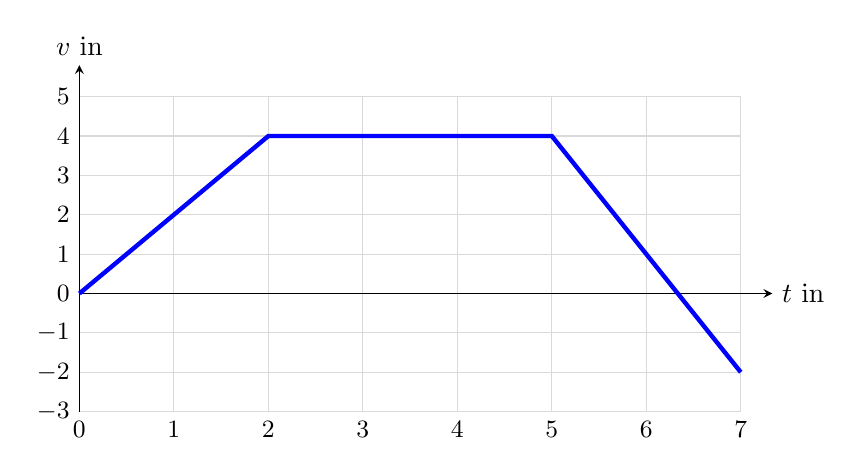
\begin{tikzpicture}[>=stealth, x=1.2cm, y=0.5cm]
 \draw[gray!30] (0,-3) grid[xstep=1, ystep=1] (7,5);
 \draw[->] (0,0) -- (7.333,0) node[right] {$t$ in \si{\second}};
 \draw[->] (0,-3) -- (0,5.8) node[above] {$v$ in \si{\meter\per\second}};
 \foreach \tk in {0,1,2,3,4,5,6,7} \node[below] at (\tk,-3) {\small $\tk$};
 \foreach \yk in {-3,-2,-1,0,1,2,3,4,5} \node[left] at (0,\yk) {\small $\yk$};
 \draw[ultra thick, blue] (0,0) -- (2,4) -- (5,4) -- (7,-2);
\end{tikzpicture}
\end{center}
\begin{abcliste}
\abc \DuSie{Skizziere}{Skizzieren Sie} das $a(t)$-Diagramm mit Werten.
\abc Lea sagt: „Am Schluss wird der Körper wieder schneller, also ist $a$ dort positiv.“ Ben sagt: „$a(t)$ hat dieselbe Form wie $v(t)$: es steigt bis \tOneO\ an, bleibt dann gleich und fällt am Ende ab.“ \DuSie{Beurteile}{Beurteilen Sie} die beiden Aussagen.
\end{abcliste}
